\documentclass{beamer}
\usepackage{tut}
\usepackage{tikz}
\usetikzlibrary{patterns}
\usepackage{pifont}
\newcommand{\xmark}{\ding{54}}%
\tikzset{onslide/.code args={<#1>#2}{%
		  \only<#1>{\pgfkeysalso{#2}} % \pgfkeysalso doesn't change the path
}}

\def\tuttitle{Rekursion, Typprüfung, Prolog}
\date{2016-12-05/06}

\begin{document}
\normalsize
\normalem

\begin{frame}[plain]
  \titlepage
\end{frame}

\begin{frame}
  \frametitle{Turing-Kombinator}
  Turing fand folgenden Fixpunktkombinator:
  \[Θ = (λ?x.~λ?y.~?y~(?x~?x~?y))~(λ?x.~λ?y.~?y~(?x~?x~?y))\]
  Zeige per $β$-Reduktion, dass gilt:
  \[Θ~F \Rightarrow^\ast F~(Θ~F)\]
\end{frame}

\begin{frame}
  \frametitle{Turing-Kombinator}
  Zur Abkürzung sei
  \begin{align*}
    Θ_0 &:= (λ?x.~λ?y.~?y~(?x~?x~?y))
    \intertext{Damit ist also}
    Θ &= Θ_0~Θ_0
    \intertext{und damit}
    Θ~F &= \onslide<2->{Θ_0~Θ_0~F} \\
    \onslide<3->{&= (λ?x.~λ?y.~?y~(?x~?x~?y))~Θ_0~F} \\
    \onslide<4->{&\Rightarrow (λ?y.~?y~(Θ_0~Θ_0~?y))~F} \\
    \onslide<5->{&\Rightarrow F~(Θ_0~Θ_0~F)} \\
    \onslide<6->{&= F~(Θ~F)}
  \end{align*}
\end{frame}

\begin{frame}
  \frametitle{Turing-Kombinator}
  Der Turing-Kombinator ist auch ein allgemeineres Rezept, um eine rekursive Gleichung zu erfüllen.
  Wollen wir etwa einen Kombinator für
  \begin{align*}
    Ξ~F &\Rightarrow^* F~(λ?g.~F~(Ξ~F~(F~Ξ)~?g))
    \intertext{so definieren wir}
    Ξ &= Ξ_0~Ξ_0
    \intertext{und definieren dann $Ξ_0$, indem wir $x$ ($Ξ_0$) und $y$ ($F$) als Parameter annehmen und dann die Rekursionsgleichung abschreiben, mit $?x~?x$ statt $Ξ$ und $?y$ statt $F$:}
    Ξ_0 &:= λ?x~λ?y.~?y~(λ?g.~?y~(?x~?x~?y~(?y~(?x~?x))~?g))
  \end{align*}
\end{frame}

\begin{frame}
  \frametitle{\vl{is\_zero}}
  Definiere Funktion \vl{is\_zero}, die prüft, ob übergebene Church-Zahl 0 ist.
  Rückgabe soll ein Church-Boolean sein, also $\ctrue$ oder $\cfalse$.
  
  \pause
  Erinnerung: eine Church-Zahl wird mit einer Nachfolgerfunktion und einem Startelement aufgerufen
  und ruft dann die Nachfolgerfunktion $n$~mal auf dem Startelement auf.
  Eine allgemeine Operation auf einer Church-Zahl hat also die Form
  \[λ?n.~?n~s~z\]
  für bestimmte $s$ und $z$.
  
  \pause
  $c_0$ gibt direkt das Startelement zurück,
  das sollte bei uns also $\ctrue$ sein.
  Wenn die Nachfolgerfunktion jemals aufgerufen wird,
  dann war die Zahl nicht 0,
  also geben wir in diesem Fall immer $\cfalse$ zurück.
  \[\vl{is\_zero} = λ?n.~?n~\underbrace{(λ?x.~\cfalse)}_{s}~\underbrace{\ctrue}_{z}\]
\end{frame}

\begin{frame}
  \frametitle{\vl{less\_eq}}
  Definiere Vergleichsfunktion \vl{less\_eq}.
  (Hier und im Rest der Aufgabe dürfen alle bisher definierten Funktionen verwendet werden.)
  \pause
  \[\vl{less\_eq} = λ?m.~λ?n.~\vl{is\_zero}~(\vl{sub}~?m~?n)\]
  (Es gibt keine negativen Church-Zahlen, daher ist z.\,B. $\vl{sub}~c_3~c_5 \Rightarrow^\ast c_0$.)
\end{frame}

\begin{frame}[fragile]
  \frametitle{\vl{fib}}
  Übersetze folgende Haskell-Funktion in $λ$-Kalkül:
  \begin{lstlisting}
    fib :: Integer -> Integer
    fib 0 = 1
    fib 1 = 1
    fib n = fib (n - 1) + fib (n - 2)
  \end{lstlisting}
\end{frame}

\begin{frame}[fragile]
  \frametitle{\vl{fib}}
  \begin{lstlisting}
    fib :: Integer -> Integer
    fib 0 = 1
    fib 1 = 1
    fib n = fib (n - 1) + fib (n - 2)
  \end{lstlisting}
  Erster Schritt: \lstinline{fib} ohne Pattern Matching.
  \pause
  \begin{lstlisting}
    fib n = if n == 0 || n == 1
            then 1
            else fib (n - 1) + fib (n - 2)
  \end{lstlisting}
\end{frame}

\begin{frame}[fragile]
  \frametitle{\vl{fib}}
  \begin{lstlisting}
    fib n = if n == 0 || n == 1
            then 1
            else fib (n - 1) + fib (n - 2)
  \end{lstlisting}
  Zweiter Schritt: zugehöriges Funktional (also ohne Rekursion) in Haskell.
  \pause
  \begin{lstlisting}
    Fib = \fib -> \n -> if n == 0 || n == 1
                        then 1
                        else fib (n - 1) + fib (n - 2)
  \end{lstlisting}
\end{frame}

\begin{frame}[fragile]
  \frametitle{\vl{fib}}
  \begin{lstlisting}
    Fib = \fib -> \n -> if n == 0 || n == 1
                        then 1
                        else fib (n - 1) + fib (n - 2)
  \end{lstlisting}
  Dritter Schritt: \lstinline{Fib} im Lambda-Kalkül.
  \pause
  \begin{align*}
    \vl{Fib} = λ\vr{fib}.~λ\vr{n}.~&(\vl{is\_zero}~(\vl{pred}~\vr{n}))\\
    &c_1\\
    &(\vl{plus}~(\vr{fib}~(\vl{sub}~\vr{n}~c_1))~(\vr{fib}~(\vl{sub}~\vr{n}~c_2)))
  \end{align*}
\end{frame}

\begin{frame}
  \frametitle{\vl{fib}}
  \begin{align*}
    \vl{Fib} = λ\vr{fib}.~λ?n.~&(\vl{is\_zero}~(\vl{pred}~?n))\\
    &c_1\\
    &(\vl{plus}~(\vr{fib}~(\vl{sub}~?n~c_1))~(\vr{fib}~(\vl{sub}~?n~c_2)))
  \end{align*}
  Vierter Schritt: \vl{fib} definieren.
  \pause
  \[\vl{fib} = Y~\vl{Fib}\]
\end{frame}

\begin{frame}
  \frametitle{Einschub: $Y$ einmal durchrechnen}
  An dieser Stelle können wir einmal das $Y$ komplett durchrechnen
  und sehen, an welcher Stelle die Rekursion passiert.
  \begin{align*}
    \vl{Fac} &= (λ\vr{fac}.~λ?n.~(\vl{isZero}~?n)~c_1~(\vl{mul}~?n~(\vr{fac}~(\vl{pred}~?n)))) \\
    Y &= λ?f.~(λ?x.~?f~(?x~?x))~(λ?x.~?f~(?x~?x)) \\
    \vl{fac} &= Y~\vl{Fac}
  \end{align*}
  Mit $\vl{fac}~c_1$ sehen wir einen Rekursionsschritt und dann den Rekursionsabbruch.
\end{frame}

\begin{frame}[fragile]
  \frametitle{\vl{foo}}
  Übersetze folgende Haskell-Funktion in $λ$-Kalkül:
  \begin{lstlisting}
    foo :: Integer -> Integer
    foo n
      | n <= 100  = foo (foo (n + 11))
      | otherwise = n - 10
  \end{lstlisting}
\end{frame}

\begin{frame}[fragile]
  \frametitle{\vl{foo}}
  \begin{lstlisting}
    foo n = if n <= 100
            then foo (foo (n + 11))
            else n - 10
  \end{lstlisting}
  Funktional:
  \pause
  \begin{lstlisting}
    Foo = \foo -> \n -> if n <= 100
                        then foo (foo (n + 11))
                        else n - 10
  \end{lstlisting}
  Funktional im Lambda-Kalkül:
  \pause
  \begin{align*}
    \vl{Foo} = λ\vr{foo}.~λ\vr{n}.~&(\vl{less\_eq}~\vr{n}~c_{100})\\
    &(\vr{foo}~(\vr{foo}~(\vl{plus}~\vr{n}~c_{11})))\\
    &(\vl{sub}~\vr{n}~c_{10})
  \end{align*}
  \vl{foo} im Lambda-Kalkül:
  \pause
  \[\vl{foo} = Y~\vl{Foo}\]
\end{frame}

\begin{frame}[fragile]
  \frametitle{\vl{foo}}
  Laut Beispiellösung ist \lstinline{foo} übrigens „die bekannte McCarthy 91-Funktion“,
  welche laut Wikipedia ein Standard-Testfall für formale Beweissysteme ist.
  Ein Beweissystem soll dabei herausfinden, dass diese Funktion die folgende Eigenschaft besitzt:
  \[\vl{foo}(n) = \begin{cases}91 & n \leq 100 \\ n - 10 & n > 100\end{cases}\]
  Daher ist \lstinline{foo} „bekanntlich“ äquivalent zu folgender Definition:
  \begin{lstlisting}
    foo n = if n <= 100 then 91 else n - 10
  \end{lstlisting}
  Damit wäre auch folgende Übersetzung denkbar:
  \[\vl{foo} = λ\vr{n}.~(\vl{less\_eq}~\vr{n}~c_{100})~c_{91}~(\vl{sub}~\vr{n}~c_{10})\]
\end{frame}

\begin{frame}[fragile]
  \frametitle{Rekursionsoperator in Haskell}
  $Y$ ist in Haskell nicht typisierbar.
  Es lässt sich aber ein anderer Rekursionsoperator definieren:
  \begin{lstlisting}
    fix :: (t -> t) -> t
    fix f = f (fix f)
  \end{lstlisting}
  (Findet sich so auch im Modul \lstinline{Data.Function}.)
  
  Definiere damit
  \begin{lstlisting}
    fibF :: (Integer -> Integer) -> (Integer -> Integer)
    fooF :: (Integer -> Integer) -> (Integer -> Integer)
  \end{lstlisting}
  sodass \lstinline{fix fibF}, \lstinline{fix fooF} die gewünschten Funktionen ergeben.
\end{frame}

\begin{frame}[fragile]
  \frametitle{\lstinline{fibF}}
  \begin{lstlisting}
    fib      :: Integer -> Integer
    fib      0 = 1
    fib      1 = 1
    fib      n = fib (n - 1) + fib (n - 2)
  \end{lstlisting}
  \pause
  \begin{lstlisting}
    fibF :: (Integer -> Integer) -> (Integer -> Integer)
    fibF _   0 = 1
    fibF _   1 = 1
    fibF fib n = fib (n - 1) + fib (n - 2)
  \end{lstlisting}
\end{frame}

\begin{frame}[fragile]
  \frametitle{\lstinline{fooF}}
  \begin{lstlisting}
    foo :: Integer -> Integer
    foo     n
      | n <= 100  = foo (foo (n + 11))
      | otherwise = n - 10
  \end{lstlisting}
  \pause
  \begin{lstlisting}
    fooF :: (Integer -> Integer) -> (Integer -> Integer)
    fooF foo n
      | n <= 100  = foo (foo (n + 11))
      | otherwise = n - 10
  \end{lstlisting}
\end{frame}

\begin{frame}
  \frametitle{Let-Polymorphismus}
  Wir wollen den folgenden Ausdruck typisieren:
  \[λ?g.~?g~(f~1)~(f~\xtrue)\]
  Dabei sei $f=λ?x.~?x$.
  
  \pause
  Intuitiv sehen wir: $f$ ist die Identitätsfunktion,
  also hat $f~1$ den Typ $\Tint$ und $f~\xtrue$ den Typ $\Tbool$.
  Damit sollte der ganze Ausdruck den Typ $(\Tint → \Tbool → α) → α$ haben.
  
  \pause
  Was ist hierbei aber der Typ von $f$?\ 
  Erster Ansatz:
  \[(λ?f.~λ?g.~?g~(?f~1)~(?f~\xtrue))~(λ?x.~?x)\]
  Dabei hat in $λ?g.~?g~(?f~1)~(?f~\xtrue)$ $?f$ den Typ $α → α$.
  Damit ist der Ausdruck aber nicht typisierbar, denn $α$ kann nicht gleichzeitig $\Tint$ und $\Tbool$ sein!
\end{frame}

\begin{frame}
  \frametitle{Let-Polymorphismus}
  Stattdessen:
  \[\Let ?f = λ?x.~?x \In λ?g.~?g~(?f~1)~(?f~\xtrue)\]
  Jetzt hat $?f$ innerhalb von $λ?g.~?g~(?f~1)~(?f~\xtrue)$ den Typ:
  \[∀α. α → α\]
  \pause
  Unterschied zu $α → α$:
  Ohne $∀$ ist $α$ eine von außen vorgegebene Typvariable,
  die für \emph{einen} Typ steht.
  Wir garantieren der Umgebung, dass wir für beliebige Belegung von $α$ funktionieren.
  Mit $∀$ dürfen wir $α$ \emph{selbst} frei wählen, beliebig oft,
  und die Umgebung garantiert \emph{uns},
  dass die Funktion vom Typ $∀ α. α → α$ für beliebige (von uns gewählte) Belegung von $α$ funktioniert.
\end{frame}

\begin{frame}[fragile]
  \frametitle{Let-Polymorphismus}
  Das gleiche gibt es übrigens auch in Haskell.
  Normalerweise ist diese Funktion nicht typisierbar:
  \begin{lstlisting}
    x f g = g (f 1) (f True)
  \end{lstlisting}
  Mit einer Language Extension wie \emph{Rank2Types} oder \emph{RankNTypes} können wir allerdings einen gültigen Typ angeben:
  \begin{lstlisting}
    x :: (forall a. a -> a) -> (Int -> Bool -> a) -> a
  \end{lstlisting}
  Die Funktion kann dann zum Beispiel mit \lstinline{id} aufgerufen werden:
  die freie Typvariable in \lstinline{a -> a} wird implizit allquantifiziert
  (\lstinline{id} hat implizit den Typ \lstinline{forall a. a -> a}).
  Im Lambda-Kalkül geschieht das nicht, dort muss man explizit \lstinline{let} verwenden.
\end{frame}

\begin{frame}
  \frametitle{Let-Polymorphismus}
  Änderungen an den Typisierungsregeln:
  \begin{description}
  \item[Var] erlaubt Instanziierungen. Zum Beispiel kann aus $Γ(x) = ∀ α. α → α$ der Typ $Γ \vdash x : \Tint → \Tint$ instanziiert werden, da $∀ α. α → α \succeq \Tint → \Tint$.
  \item[Abs] fordert, dass der Parametertyp kein Typschema ist.
  \item[Let] neue Regel:
    \begin{prooftree}
      \AxiomC{$Γ \vdash t_1 : τ_1$}
      \AxiomC{$Γ, ?x : \mathit{ta}(τ_1, Γ) \vdash t_2 : τ_2$}
      \rulename{Let}
      \BinaryInfC{$Γ \vdash \Let ?x = t_1 \In t_2 : τ_2$}
    \end{prooftree}
    Dabei hat $t_1$ einen normalen (nicht polymorphen) Typ, also mit freien Typvariablen, z.\,B. $α → β → α$.
    $t_2$ darf die polymorphe Version davon nutzen, hier z.\,B. $∀ α. ∀ β. α → β → α$.
    Das \lstinline{let}-Konstrukt schafft den Übergang zwischen den beiden Ausdrücken.
  \end{description}
\end{frame}

\begin{frame}
  \frametitle{Typprüfung}
  Gegeben
  \[Γ = ?a: \Tint, ?b: \Tbool, ?c: \Tchar\]
  soll unter Verwendung der folgenden Instanziierungen
  \begin{align*}
    & ∀α. ∀β. α → β → α \succeq \Tint → \Tbool → \Tint \\
    & ∀α. ∀β. α → β → α \succeq \Tbool → \Tchar → \Tbool
  \end{align*}
  der folgende Herleitungsbaum vervollständigt werden:
  
  \begin{prooftree}
    \small
    \AxiomC{$Γ \vdash λ?x.~λ?y.~?x : α → β → α$}
    \AxiomC{$Γ, ?k : ∀α. ∀β. α → β → α \vdash ?k~?a~(?k~?b~?c) : \Tint$}
    \rulename{Let}
    \BinaryInfC{$Γ \vdash \Let ?k = λ?x.~λ?y.~?x \In ?k~?a~(?k~?b~?c) : \Tint$}
  \end{prooftree}
\end{frame}

\begin{frame}
  \frametitle{Typprüfung}
  Wir zeigen zunächst die linke Seite
  \[Γ \vdash λ?x.~λ?y.~?x : α → β → α\]
  durch mehrmalige Anwendung der Regel
  \pause
  \begin{prooftree}
    \AxiomC{$Γ, ?x: τ_1 \vdash t: τ_2$}
    \rulename{Abs}
    \UnaryInfC{$Γ \vdash λ?x.~t: τ_1 → τ_2$}
  \end{prooftree}
\end{frame}

\begin{frame}
  \frametitle{Typprüfung}
  \begin{prooftree}
    \def\fCenter{(?x}
    \Axiom$(Γ, ?x: α, ?y: β)\fCenter) = α$
    \def\fCenter{\vdash}
    \rulename{Var}
    \UnaryInf$Γ, ?x:α, ?y:β \fCenter ?x: α$
    \rulename{Abs}
    \UnaryInf$Γ, ?x: α \fCenter λ?y.~?x : β → α$
    \rulename{Abs}
    \UnaryInf$Γ \fCenter λ?x.~λ?y.~?x : α → β → α$
  \end{prooftree}
\end{frame}

\begin{frame}
  \frametitle{Typprüfung}
  Jetzt zeigen wir die rechte Seite
  \[Γ, ?k : \underbrace{∀α. ∀β. α → β → α}_{ξ} \vdash ?k~?a~(?k~?b~?c) : \Tint\]
  mit der Regel
  \pause
  \begin{prooftree}
    \AxiomC{$Γ \vdash t_1: τ_2 → τ$}
    \AxiomC{$Γ \vdash t_2: τ_2$}
    \rulename{App}
    \BinaryInfC{$Γ \vdash t_1~t_2: τ$}
  \end{prooftree}
  also
  \begin{prooftree}
    \AxiomC{$Γ, ?k:ξ \vdash ?k~?a: \Tbool → \Tint$}
    \AxiomC{$Γ, ?k:ξ \vdash ?k~?b~?c: \Tbool$}
    \rulename{App}
    \BinaryInfC{$Γ, ?k:ξ \vdash ?k~?a~(?k~?b~?c) : \Tint$}
  \end{prooftree}
\end{frame}

\begin{frame}
  \frametitle{Typprüfung}
  $?k~?a$ ist auch eine Applikation, also gleiche Regel nochmal:
  \begin{prooftree}
    \AxiomC{$Γ, ?k:ξ \vdash ?k: \Tint → \Tbool → \Tint$}
    \AxiomC{$(Γ, ?k:ξ)(?a) = \Tint$}
    \rulename{Var}
    \UnaryInfC{$Γ, ?k:ξ \vdash ?a: \Tint$}
    \rulename{App}
    \BinaryInfC{$Γ, ?k:ξ \vdash ?k~?a: \Tbool → \Tint$}
  \end{prooftree}
  \onslide<2->{
    Das sind zwei Variablentypen, also zwei \textit{Var}-Regeln;
    die linke ist polymorph:
    \begin{prooftree}
      \AxiomC{$(Γ, ?k:ξ)(?k) = ξ$}
      \AxiomC{$ξ \succeq \Tint → \Tbool → \Tint$}
      \rulename{Var}
      \BinaryInfC{$Γ, ?k:ξ \vdash ?k: \Tint → \Tbool → \Tint$}
    \end{prooftree}
  }
  (Erinnerung: $ξ = ∀α. ∀β. α → β → α$)
\end{frame}

\begin{frame}
  \frametitle{Typprüfung}
  Die verbleibende Beweisverpflichtung ist
  \[Γ, ?k:ξ \vdash ?k~?b~?c: \Tbool\]
  \pause
  Zweimal \textit{App}, zweimal \textit{Var}:
  \begin{prooftree}
    \AxiomC{$Γ, ?k:ξ \vdash ?k~?b: \Tchar → \Tbool$}
    \AxiomC{$(Γ, ?k:ξ)(?c) = \Tchar$}
    \rulename{Var}
    \UnaryInfC{$Γ, ?k:ξ \vdash ?c: \Tchar$}
    \rulename{App}
    \BinaryInfC{$Γ, ?k:ξ \vdash ?k~?b~?c: \Tbool$}
  \end{prooftree}
  \begin{prooftree}
    \AxiomC{$Γ, ?k:ξ \vdash ?k: \Tbool → \Tchar → \Tbool$}
    \AxiomC{$(Γ, ?k:ξ)(?b) = \Tbool$}
    \rulename{Var}
    \UnaryInfC{$Γ, ?k:ξ \vdash ?b: \Tbool$}
    \rulename{App}
    \BinaryInfC{$Γ, ?k:ξ \vdash ?k~?b: \Tchar → \Tbool$}
  \end{prooftree}
\end{frame}

\begin{frame}
  \frametitle{Typprüfung}
  Und für den Beweis von
  \[Γ, ?k:ξ \vdash ?k: \Tbool → \Tchar → \Tbool\]
  verwenden wir erneut die polymorphe Variante der \textit{Var}-Regel:
  \begin{prooftree}
    \AxiomC{$(Γ, ?k:ξ)(?k) = ξ$}
    \AxiomC{$ξ \succeq \Tbool → \Tchar → \Tbool$}
    \BinaryInfC{$Γ, ?k:ξ \vdash ?k: \Tbool → \Tchar → \Tbool$}
  \end{prooftree}
  ($ξ$ ist immer noch $∀α. ∀β. α → β → α$.)
\end{frame}

\prolog

\begin{frame}[fragile]
  \frametitle{Prolog}
  Ein Prolog-Programm besteht aus wahren Aussagen, nämlich Fakten und Regeln.
  \begin{lstlisting}
    person(thomas).
    person(michelle).
    person(john).
    mutter(michelle, thomas).
    vater(john, thomas).
    elter(X,Y) :- mutter(X,Y); vater(X,Y).
    grosselter(X,Y) :- elter(X,Z), elter(Z,Y).
  \end{lstlisting}
  Kleingeschriebene Namen sind Atome, großgeschriebene Variablen.
  Fakten enden mit einem Punkt,
  Regeln listen die Bedingungen nach einem \lstinline{:-} auf.
  Dabei werden Bedingungen durch \lstinline{,} (und) oder \lstinline{;} (oder) getrennt.
  Oder-Regeln werden aber üblicherweise geschrieben als
  \begin{lstlisting}
    elter(X,Y) :- mutter(X,Y).
    elter(X,Y) :- vater(X,Y).
  \end{lstlisting}
\end{frame}

\begin{frame}[fragile]
  \frametitle{Prolog}
  Die Benutzung von Prolog besteht darin, Anfragen zu stellen:
  \begin{lstlisting}
    ?- person(thomas).
    true.
    
    ?- person(smith).
    false.
  \end{lstlisting}
  Prolog durchsucht dann die bekannten Aussagen, um die Anfrage zu überprüfen.
  
  Eine Anfrage kann auch freie Variablen enthalten,
  Prolog versucht dann immer wieder, die Aussage zu erfüllen.
  \begin{lstlisting}
    ?- person(X).
    X = thomas ;
    X = michelle ;
    X = john.
  \end{lstlisting}
\end{frame}

\begin{frame}[fragile]
  \frametitle{Prolog}
  Listen funktionieren ähnlich wie in Haskell (leere Liste, Cons), nur mit anderer Syntax.
  Cons wird geschrieben als \lstinline{[X|Y]}, wobei \lstinline{X} ein Element und \lstinline{Y} die Rest-Liste ist.
  \lstinline{[1,2,3]} steht also für \lstinline{[1|[2|[3|[]]]]}.
\end{frame}

\begin{frame}[fragile]
  \frametitle{Prolog}
  \begin{lstlisting}
    e(x1).
    e(x2).
    f(x1).
    f(x2).
    g(x1).
    g(x2).
    a(X) :- e(X), f(X),    g(X).
  \end{lstlisting}
\end{frame}

\begin{frame}[fragile]
  \makeatletter
  \newcommand*{\overlaynumber}{\number\beamer@slideinframe}
  \makeatother
  \begin{overprint}
  \onslide<1>
    \begin{lstlisting}[language=Prolog,gobble=4,mathescape]
      a(x) :- e(x), f(x), $\phantom{\textbf{!,}}$ g(x).
    \end{lstlisting}
  \onslide<2->
    \begin{lstlisting}[language=Prolog,gobble=4,mathescape]
      a(x) :- e(x), f(x), $\textbf{!,}$ g(x).
    \end{lstlisting}
  \end{overprint}

  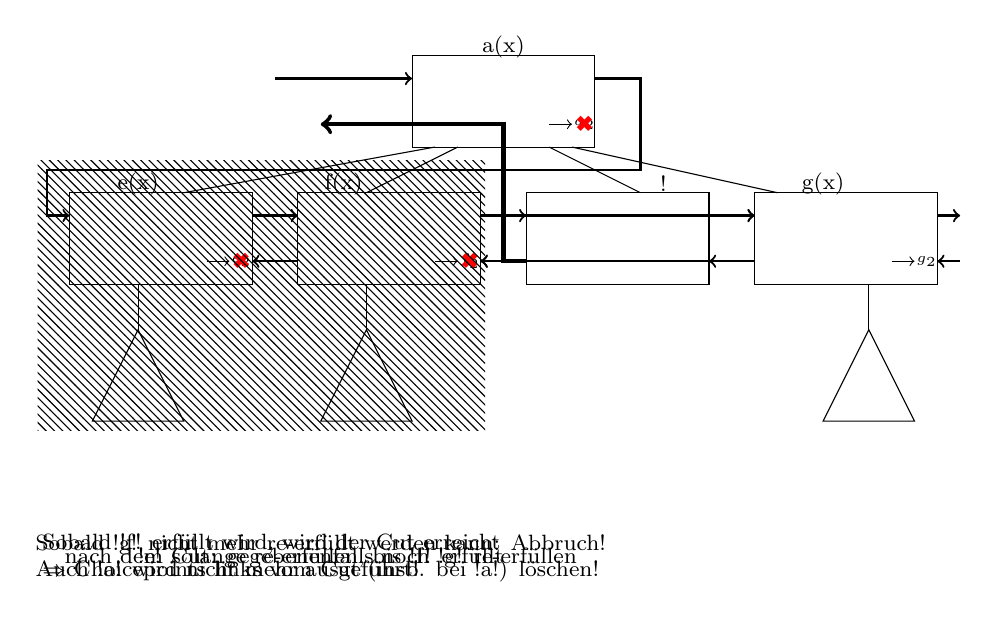
\begin{tikzpicture}[scale=.58]
  % boxes
  \draw (0,0) -- (4,0) -- (4,2) -- (0,2) -- cycle;
  \draw[xshift=-7.5cm,yshift=-3cm] (0,0) -- (4,0) -- (4,2) -- (0,2) -- cycle;
  \draw[xshift=-2.5cm,yshift=-3cm,onslide=<2>{thick}] (0,0) -- (4,0) -- (4,2) -- (0,2) -- cycle;
  \draw<2->[xshift= 2.5cm,yshift=-3cm,onslide=<3>{thick}] (0,0) -- (4,0) -- (4,2) -- (0,2) -- cycle;
  \draw[xshift= 7.5cm,yshift=-3cm] (0,0) -- (4,0) -- (4,2) -- (0,2) -- cycle;
  \draw (-6,-4) -- (-7,-6) -- (-5,-6) -- cycle;
  \draw[xshift=5cm] (-6,-4) -- (-7,-6) -- (-5,-6) -- cycle;
  \draw[xshift=16cm] (-6,-4) -- (-7,-6) -- (-5,-6) -- cycle;

  % choice points
  \draw<1,2,3,4,5>[->] (3,0.5)  -- (3.5,0.5) node[anchor=west,xshift=-0.1cm] (cp-a) {\tiny $a_2$};
  \draw<1,2,3,4,5>[->,xshift=-7.5cm,yshift=-3cm] (3,0.5) -- (3.5,0.5) node[anchor=west,xshift=-0.1cm] (cp-e) {\tiny $e_2$};
  \draw<1,3,4,5>[->,xshift=-2.5cm,yshift=-3cm] (3,0.5) -- (3.5,0.5) node[anchor=west,xshift=-0.1cm] (cp-f) {\tiny $f_2$};
  \draw<1,4>[->,xshift=7.5cm,yshift=-3cm] (3,0.5) -- (3.5,0.5) node[anchor=west,xshift=-0.1cm] (cp-g) {\tiny $g_2$};


  % child-relations
  \draw (0.5,0) -- (-5,-1);
  \draw (1,0) -- (-1,-1);
  \draw<2-> (3,0) -- (5,-1);
  \draw (3.5,0) -- (8,-1);
  \draw (-6,-3) -- (-6,-4);
  \draw (-1,-3) -- (-1,-4);
  \draw (10,-3) -- (10,-4);
  % control flow
  \draw[->,thick] (-3,1.5) -- (0,1.5);
  \draw[->,thick] (4,1.5) -- (5,1.5) -- (5,-0.5) -- (-8,-0.5) -- (-8,-1.5) -- (-7.5,-1.5);
  \draw[->,thick] (-3.5,-1.5) -- (-2.5,-1.5);
  \draw[<-,thick] (-3.5,-2.5) -- (-2.5,-2.5);
  \draw<1>[->,thick] (1.5,-1.5) -- (7.5,-1.5);
  \draw<2->[->,thick] (1.5,-1.5) -- (2.5,-1.5);
  \draw<2->[->,thick] (6.5,-1.5) -- (7.5,-1.5);
  \draw<2->[<-,thick] (6.5,-2.5) -- (7.5,-2.5);
  \draw[->,thick] (11.5,-1.5) -- (12,-1.5);
  \draw[<-,thick] (11.5,-2.5) -- (12,-2.5);
  \draw<1>[->,thick] (7.5,-2.5) -- (1.5,-2.5);
  \draw<2>[->,thick] (2.5,-2.5) -- (1.5,-2.5);
  \draw<5->[->,ultra thick] (2.5,-2.5) -- (2,-2.5) -- (2,0.5) -- (-2,0.5);

  % box labels
  \footnotesize
  \node at (2,2.2) {a(x)};
  \node at (-6,-0.8) {e(x)};
  \node at (-1.5,-0.8) {f(x)};
  \node<2-> at ( 5.5,-0.8) {!};
  \node at (9,-0.8) {g(x)};

  % eliminate choice points
  \node<3-> at (cp-a) {\textcolor{red}{\xmark}};
  \node<3-> at (cp-e) {\textcolor{red}{\xmark}};
  \node<3-> at (cp-f) {\textcolor{red}{\xmark}};

  % for debugging purposes: show current overlay number
  %\node at (10,-10) {\overlaynumber};

  \onslide<2>{\node[anchor=center] at (-2, -9) {\lstinline!e! solange re-erfüllen, bis \lstinline!f! erfüllt};}
  \onslide<3>{\node[anchor=center,align=left] at (-2, -9) {Sobald \lstinline!f! erfüllt wird, wird der Cut erreicht \\$\Rightarrow$ Choicepoints links vom Cut (insb. bei \lstinline!a!) löschen!};}
  \onslide<4>{\node[anchor=center] at (-2, -9) {nach dem Cut: gegebenenfalls noch \lstinline!g! re-erfüllen};}
  \onslide<5>{\node[anchor=center,align=left] at (-2, -9) {Sobald \lstinline!g! nicht mehr re-erfüllt werden kann: Abbruch! \\Auch \lstinline!a! wird nicht mehr ausgeführt!};}
  % strike through
  \usetikzlibrary{patterns};
  \onslide<5->{\fill[pattern=north west lines] (-8.2,-0.3) rectangle (1.6,-6.2);}


  \end{tikzpicture}
\end{frame}

\end{document}
